
Nel seguente capitolo  verrà fatto un excursus su tutte le tecnologie scelte per lo sviluppo della base di dati a grafo e della API RESTful di questo progetto di tesi, con particolare focus sugli gli strumenti utilizzati per la gestione dell'architettura client-server, compreso il trasferimento di informazioni tra essi.

\subsection{Neo4j e driver di collegamento}

Al giorno d'oggi uno dei graph database pù conosciuti  è \emph{Neo4j}. Implementato in Java, permette la creazione di strutture dati organizzate in grafi anzichè tabelle.
Garantisce la scalabilità orizzontale dei dati, permettendone l'aggiunta di nuovi in maniera semplice, fornendo anche un'interfaccia grafica molto intuitiva per la loro visualizzazione  \cite{Graph-neo4j-analysis}.

\emph{Cypher} \cite{neo4j} è il linguaggio dichiarativo, nativo utilizzato da Neo4j.
Tramite il quale si possono scrivere interrogazioni in modo più immediato.
Con la clausola \emph{MATCH} è possibile individuare sia entità che relazioni allo stesso tempo.
Per determinati aspetti è molto simile al linguaggio SQL, soprattutto per quanto riguarda la clausola \emph{WHERE}, utilizzata principalmente per filtrare i risultati. L'ordine di scrittura delle query è pressoché identico.
I risultati delle query  vengono mostrati attraverso in'interfaccia che offre una panoramica compatta e intuitiva dei dati richiesti.

Per permettere l'utilizzo queste informazioni ad utenti con altre necessità d'uso, si può usufruire dei driver ufficiali di Neo4j.
In questo progetto di tesi, sono stati utilizzati quelli compatibili con JavaScript, tramite i quali è possibile definire un'istanza utile ad instaurare una connessione ad un server che ospita un database Neo4j.
La sessione viene stabilita tramite l'uso di un URI e credenziali di autorizzazione e può essere effettuata attraverso l'utilizzo di due possibili protocolli: neo4j e bolt.

Il primo risulta molto efficace quando si ha la necessità di avere a disposizione un servizio di routing automatico delle query verso il nodo appropriato di un cluster di server.
Il secondo, usato per il progetto di tesi, è la scelta più utilizzata quando si parla di connessione ad un server neo4j remoto, in quanto in grado di effettuare una connessione diretta ad un singolo server, garantendo efficienza, velocità e riduzione della latenza nella comunicazione.
Una volta instaurata la connessione, è possibile inoltrare al server delle query scritte in Cypher tramite il driver, il quale è in grado di restituire un riepilogo contenente alcuni dettagli sulle interrogazioni effettuate come il loro tipo, o se presenti le modifiche apportate al database.



\subsection{Express framework e Node.js}
\emph{Express} \cite{ex-express} è il framework standard de facto per lo sviluppo di infrastrutture web, scritto in Javascript utilizzabile con Node.js che consiste in un insieme di strumenti per la gestione di richieste e risposte HTTP e routing, utili allo sviluppo di qualsiasi applicativo web. 

\emph{Node.js} \cite{mdn-express} è un ambiente di \textit{run-time}, open-source e capace di funzionare su piattaforme diverse, utile per l'esecuzione di codice in linguaggio Javascript e lo sviluppo di applicazioni server-side. Tramite il package manager \emph{npm} è possibile installare librerie sviluppate da utenti in tutto il mondo, con le quali ampliare le funzionalità delle web application.

L'integrazione di Express permette la risoluzione di alcuni task di programmazione web, altrimenti non risolvibili con il solo utilizzo delle funzionalità native di Node.js, come la gestione delle operazioni CRUD.

Le operazioni \emph{CRUD} \cite{Martin1983ManagingTD} sono fondamentali per la gestione persistente dei dati all'interno di un database: create(creazione), read(lettura), update(aggiornamento), delete(cancellazione).
Le loro trasposizioni in contesti legati alle web API non sono altro che i metodi HTTP, ovvero \emph{GET, POST, PUT e UPDATE}.

Express infatti gestisce in modo più efficace queste operazioni, permettendo la gestione separata di tali richieste, tramite l'utilizzo di diversi \emph{URL}. 
Inoltre con l'uso di middleware è possibile estendere le sue funzionalità, tra cui la gestione dei cookie, degli accessi da parte degli utenti o anche del caching.
La sua velocità e la sua struttura minimalista gli permettono di essere la scelta più popolare tra gli sviluppatori che hanno a che fare con progetti legati alle API.

\thispagestyle{mystyle}
\subsection{XMLHttpRequest}
\emph{XMLHttpRequest} \cite{mdn-XMLHttpRequest} è un oggetto Javascript tipicamente utilizzato lato client, per interagire con i server. Con i metodi messi a disposizione si possono effettuare delle richieste ad un determinato URL, e riceverne le corrispondenti risposte.
La possibilità di gestione asincrona di queste ultime, rende possibile l'esecuzione di altre parti di codice mentre si è in attesa delle risposte da parte del  server.
Inoltre ciò rende possibile l'aggiornamento dinamico della pagina web, senza avere la necessità di ricaricarla per intero.

La gestione dei parametri della comunicazione attuata tramite questo oggetto è affidata all'utilizzo di parametri fondamentali, tra cui:

\begin{itemize}
    \item  \emph{responseType}: proprietà che permette di specificare il tipo di dato della risposta da parte del server.
    I tipi che possono essere selezionati sono molteplici, tra cui anche dati in formato testuale e JSON.

    \item \emph{status}: proprietà di sola lettura in grado di restituire un codice numerico identificativo dello stato della risposta HTTP del server. I valori restituiti possono essere 0 per \emph{UNSENT} e \emph{OPENED} in caso di richiesta ancora non gestita, oppure 200 per \emph{LOADING} e \emph{DONE} in caso di richiesta correttamente gestita.
    
    \item \textit{statusText}: proprietà di sola lettura che restituisce un messaggio riguardante lo stato della richiesta HTTP.
    A differenza del parametro precedente, contiene del testo, come ad esempio "OK" o "Not Found".

    \item \textit{timeout}: tempo, in millisecondi, dopo il quale una richiesta viene automaticamente annullata.
\end{itemize}


L'inizializzazione delle richieste avviene attraverso l'utilizzo del metodo \emph{open()}.
Tramite tale metodo si possono definire i parametri di tali richieste, tra cui l'URL endpoint al quale inoltrarle e il metodo HTTP usato.
L'inoltro al server viene effettuato dal metodo \emph{send()}.
Di fondamentale importanza è la gestione degli eventi quando si ha a che fare con una comunicazione client-server.
Attraverso alcune proprietà particolari si possono gestire determinati eventi che si presentano, tra cui \emph{onload}, il quale si attiva quando si ottiene una risposta dal server e può essere utilizzato per verificarne la corretta esecuzione o la presenza di errori nella gestione.

\thispagestyle{mystyle}
\subsection{JSON}
Il \emph{JSON} (JavaScript Object Notation) \cite{JsonDocs} è un formato utilizzato per lo scambio di dati, basato sul linguaggio JavaScript, facilmente interpretabile da esseri umani e macchine.
Nonostante la completa indipendenza dai vari linguaggi di programmazione, l'utilizzo di convenzioni comuni ad essi, lo rende il formato ideale per lo scambio di informazioni.
Di seguito è riportato un esempio di oggetto JSON:

\begin{figure}[H]
    \centering
    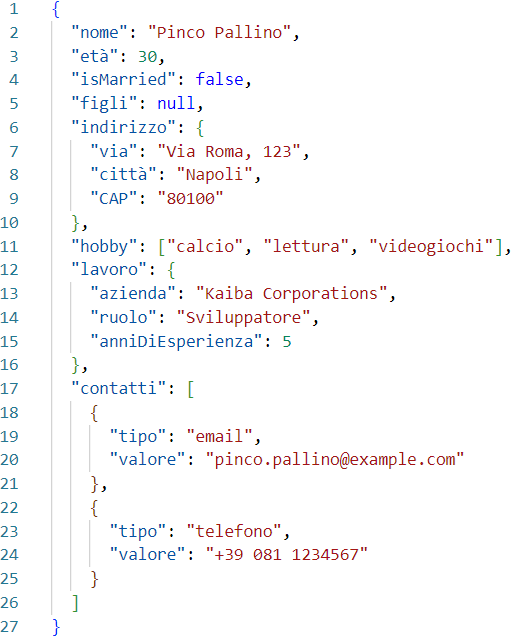
\includegraphics[keepaspectratio=true,scale=0.5]{Images/JSONExample.png}
    \caption{Esempio di oggetto JSON}
\end{figure}


Per indicare l'inizio e la fine di un oggetto vengono utilizzate le parentesi graffe (riga 1 e 27).
L'oggetto in questione utilizza la seguente rappresentazione
\begin{center}
   \emph{"chiave": valore}
\end{center}
 equiparabile ad una tavola hash o un dizionario negli ordinari linguaggi di programmazione.
 Se il valore è delimitato da virgolette allora si tratta di una stringa (riga 2), in caso contrario si tratta di un tipo primitivo (riga 3).
 Possono essere definiti anche valori nulli utilizzando la parola chiave \emph{null} (riga 5) o valori booleani (riga 4).
Inoltre è possibile rappresentare anche degli array semplici e quindi composti da singoli elementi (riga 11) oppure array complessi, nel quale ogni elemento possiede più attributi (da riga 17 a riga 26). La virgola viene utilizzata come carattere separatore degli attributi.

\thispagestyle{mystyle}

\subsection{Swagger}
\emph{Swagger} \cite{Swagger} mette a disposizione un insieme di software utili per progettare, sviluppare, documentare e testare API RESTful. Il punto saliente è la possibilità di generare una documentazione interattiva, facilitando la comprensione da parte degli sviluppatori e degli utilizzatori di tali API.
Tramite un'interfaccia grafica intuitiva, generata ad un determinato endpoint (ad esempio \emph{/api-docs}), è possibile  effettuare degli adeguati test utili a verificarne la correttezza.
Nello specifico i test di cui sopra tendono a verificare la corretta gestione delle chiamate che vengono effettuate ai server, mostrando all'utente una risposta o un eventuale errore.

La documentazione segue la specifica \textit{OpenAPI} che definisce uno standard per la documentazione delle API, in modo da renderle comprensibili, senza avere la necessità di leggere il codice sorgente.

L'insieme dei software messi a disposizione comprende:
\begin{itemize}
    \item \emph{Swagger Editor}: un editor online che permette agli sviluppatori di scrivere o modificare le API scritte seguendo le specifiche OpenAPI di cui sopra.
    \item \emph{Swagger UI}: installabile tramite npm, permette di generare una documentazione interattiva, attraverso la quale effettuare dei test.

    \item \emph{Swagger Codegen}: strumento in grado di generare in autonomia dei client \emph{SDK} (Software Development Kit) o server stubs (codice di base per i server), per permettere l'integrazione delle API nelle diverse applicazioni degli sviluppatori.

    \item \emph{Swagger Inspector}: strumento utile per testare o estrarre specifiche OpenAPI da API già esistenti.
\end{itemize}

Di seguito verrà mostrata un esempio di documentazione generata tramite swagger UI e \emph{swagger-jsdocs} per Javascript.

\begin{figure}[H]
    \centering 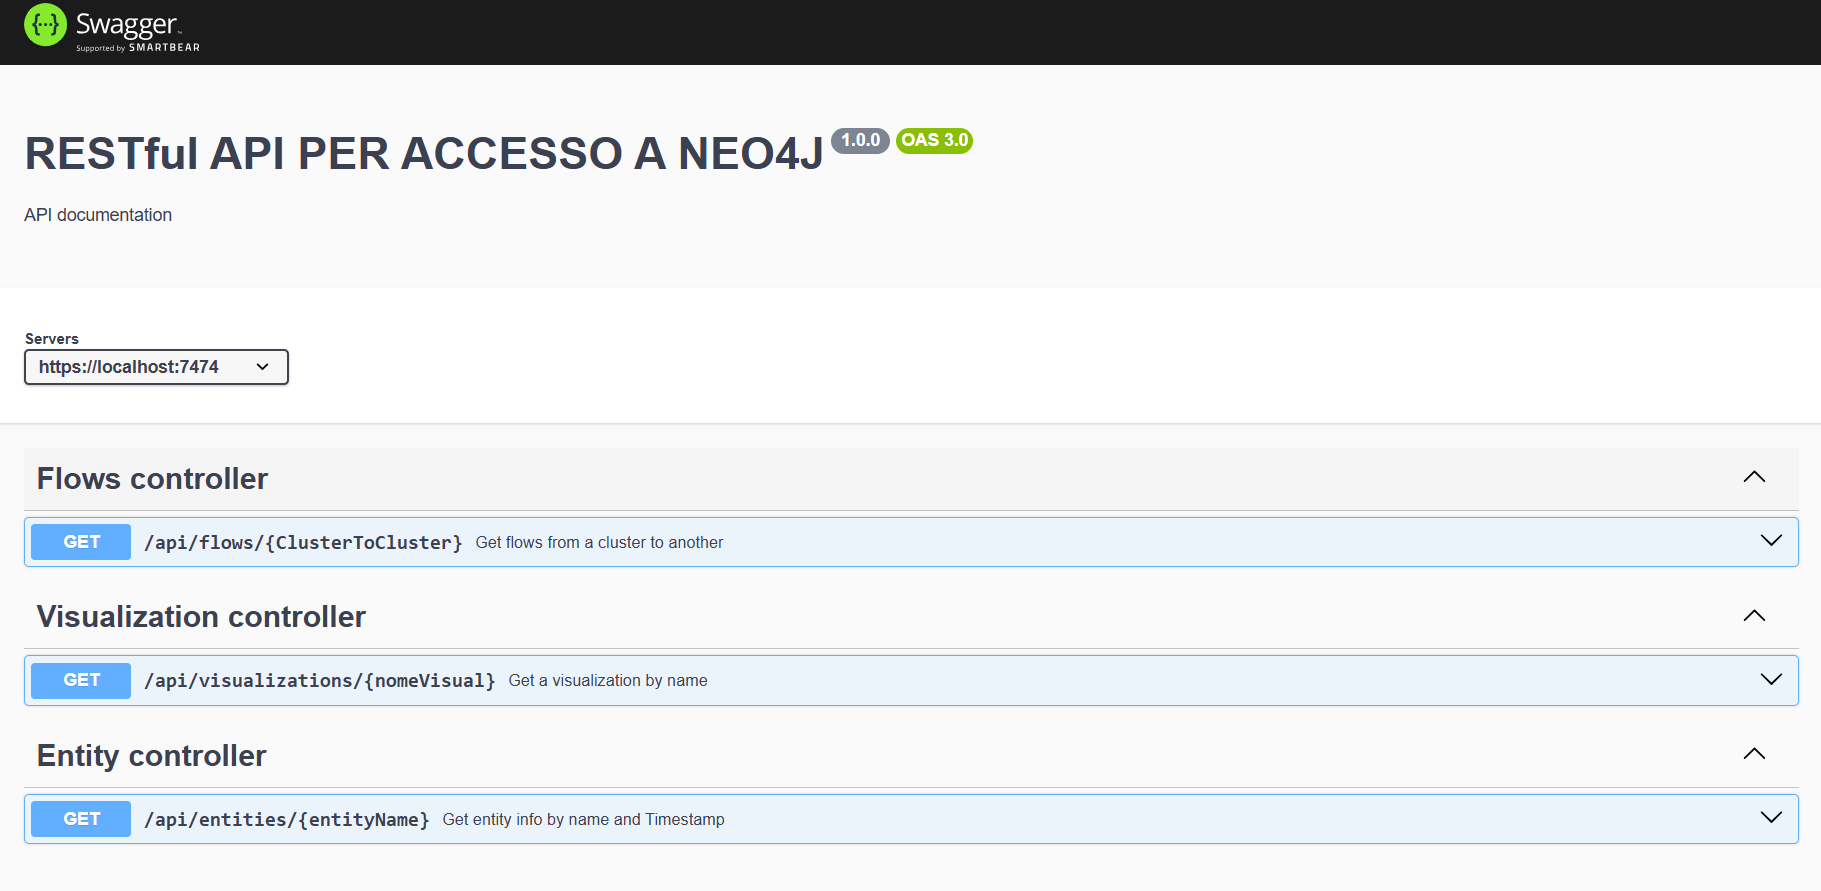
\includegraphics[keepaspectratio=true,scale=0.3]{Images/SchermataInizialeDocs.png}
    \caption{Schermata iniziale API Documentation generata con Swagger UI.}
\end{figure}

\thispagestyle{mystyle}


